\section{The steady state}
%
The steady state is achieved as described in \cref{sec:initRun}.
We will in this section discuss the shape of the resulting profiles, and the physics behind their shapes.
% FIXME: Add this somewhere:
%        Changes in profiles when increasing B:
%        Parallel:
%        - Bump in current close to sheath goes up
%        - Vort initially neg an monotonically growing, now bumped above 0
%           + Does not coincide with node in fluctuations
%        - n increases <-- confinement? Naah....most is lost in the parallel direction anyways
%        Perpendicular:
%        - Profile steepening

\subsection{Parallel profiles}
%
The resulting parallel profiles for the steady state are shown in \cref{fig:parProfs}.
%
\begin{figure}[htb]
    \centering
    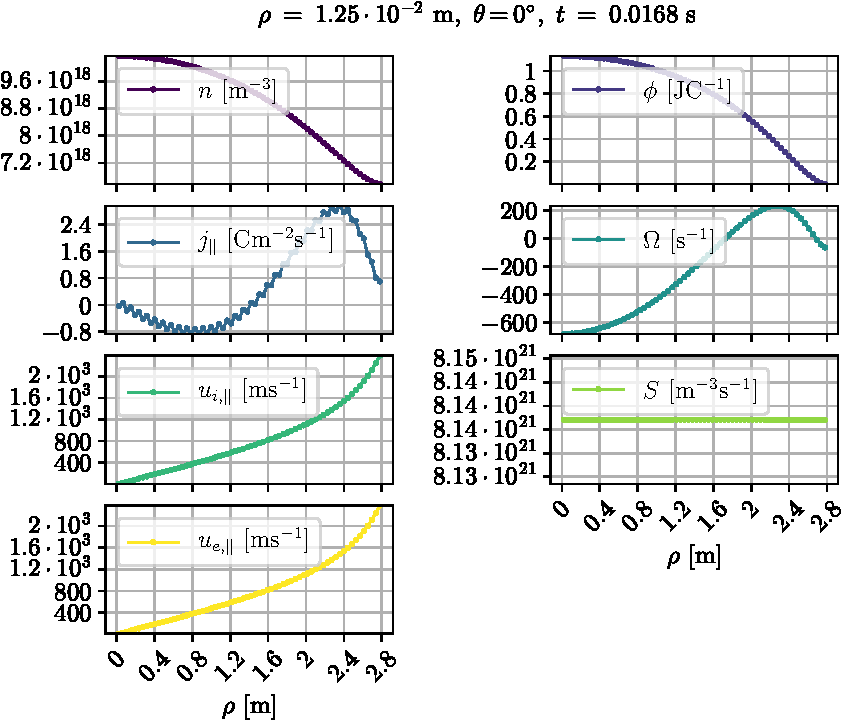
\includegraphics{fig/results/1DProfiles/B010Par}
    \caption{Parallel profiles in the steady state for $B=0.1\T$}
    \label{fig:parProfs}
\end{figure}
%
It is found that the shape of these profiles are mainly determined by the source and the boundary condition at the sheath entrance.

If we change the source amplitude, the values of the profiles changes, but the shape remain relatively constant.
There exists a threshold on the source amplitude for the filling of the plasma cylinder.
For source amplitudes under this threshold it is observed that the cylinder is "emptied" for plasma.
That is: The density remains low for all time steps, and no density profile builds up.
There also exists an upper limit on the source amplitude.
Above this threshold, the radial density profiles are not developing, and the plasma is emptied only in the parallel direction.
In between these two extremes, the parallel extent of the source determines the filling.
That is: The parallel shape of the density is determined by the parallel extent of the source, and not so much by the shape of the source itself.

As mentioned above, also the boundary condition at the sheath entrance is critical for the parallel shape of the plasma profiles.
If the boundary condition on the density is changed to for example Cauchy boundary condition (described in \cref{sec:BCatSE}), it is observed that the shape of the steady state profiles becomes much steeper close to the sheath entrance.
Gradients that steep usually gives rise to numerical instabilities, unless the spatial resolution in this area is increased.

We observe that the potential profile in \cref{fig:parProfs} follows the density profile quite well.
This is expected because:
%
\begin{enumerate}[noitemsep]
        \item The pressure is balancing the electric field to the first order, as seen in the ordering described in \ref{app:DO}.
        \item We do not restrict the potential by any parallel boundary condition.
\end{enumerate}

Next, the parallel velocity profiles are mainly arising from the parallel boundary condition.
Both the ions and electrons are fixed to a zero velocity at the boundary opposite to the sheath.
Furthermore, the ions are fixed to the ion sound velocity at the sheath entrance, whereas the electron velocity will regulate itself after the potential.
If more electrons than ions were to escape, a potential difference would build up attracting more ions and pushing away more electrons.
%
% Why is it not ambipolar?
%
Any difference in the parallel velocities would lead to parallel currents.

The divergence of current must be constant as a consequence of charge conservation.
Any parallel derivatives in the parallel current not balancing the other terms in \cref{eq:celma_vortD_evolution} would lead to an acceleration of the plasma spinning.
Therefore, the radial vorticity profile comes as a direct consequence of the parallel derivative of the current in that point.
Due to this, one should take care that the see-sawing in the parallel current profile is kept to a minimum.
The see-saw pattern seen in \cref{fig:parProfs} is at the maximum level allowed in this thesis, and arises from the poor parallel resolution mentioned in \ref{sec:resolution}.

\subsection{Radial profiles}
%
The radial profiles are shown in \cref{fig:radProfs}.
%
\begin{figure}[htb]
    \centering
    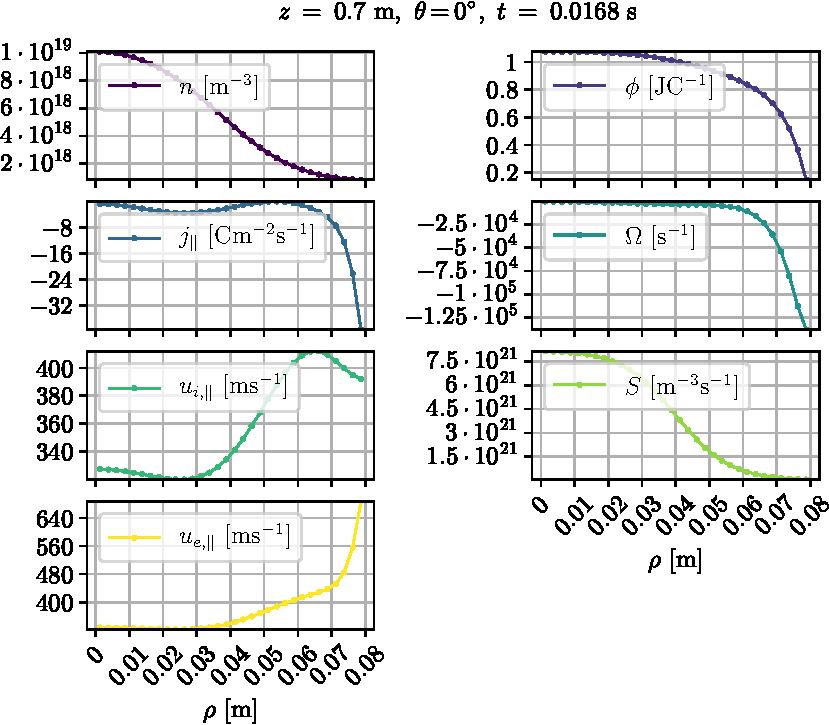
\includegraphics{fig/results/1DProfiles/B010Rad}
    \caption{Radial profiles in steady state for $B=0.1\T$}
    \label{fig:radProfs}
\end{figure}
%
As for the parallel direction, the shape of the radial density profile is determined mainly by the source and the radial boundary conditions.
The radial extent of the source plays a larger role in determining the radial density profile as compared with the shape of the source.

Despite having almost Boltzmann distributed electrons in the parallel direction at each radial point close to the axis, the Boltzmann distribution not apply in the radial direction.
This is because the plasma is confined in the parallel direction by the strong magnetic field.
Close to $L_\rho$ the radial potential profile is affected more by the fixation potential to $0$ at $L_\rho$.
Thus, the values here differs from the density profile because of the zero gradient enforcement on $n$ at $L_\rho$.
